Nesta seção, iremos apresentar os elementos necessários ao texto escrito, os itens que são obrigatórios, suas características, como organizá-los e também quais os modelos de documentos (conhecidos como \emph{templates}). Embora a estrutura apresentada não seja uma regra absoluta, ela é uma regra geral que captura o perfil destes tipos de trabalho.

\subsection{Trabalho de Conclusão de Curso I}

O Trabalho de Conclusão de Curso I (TCC1) deve ser formatado segundo o \emph{template} da Sociedade Brasileira de Computação (SBC), disponível no repositório \emph{git} em que se encontra o manual do aluno (\href{https://github.com/elloa/manual-aluno/tree/master/templates}{clique aqui para acessar}).

s elementos necessários para o TCC1 são apresentados a seguir, juntamente com alguns exemplos que os ilustram:

\begin{enumerate}
  \item \textbf{Título};
  \item \textbf{Autores}. Aluno, orientador e co-orientador, se houver;
  \item \textbf{Dados para contato}. Endereço profissional e e-mail dos autores;
\end{enumerate}

Os dados para contato dos autores idealmente devem mostrar o endereço profissional onde o trabalho está sendo desenvolvido, neste caso na Escola Superior de Tecnologia, e os e-mails para contato devem ser os e-mails institucionais. Se possível, os e-mails devem ser agrupados para uma melhor visualização. A Figura \ref{fig:cabecalhoTCC1} ilustra um exemplo destes elementos que compõem o cabeçalho do TCC1.

\begin{figure}[h!]
  \centering
\fbox{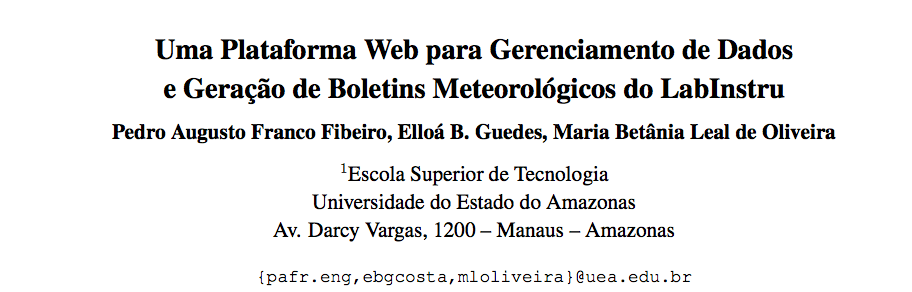
\includegraphics[width=0.8\textwidth]{./img/exemplo-cabecalho-tcc1}}\caption{Exemplo de cabeçalho do TCC1.}  \label{fig:cabecalhoTCC1}
\end{figure}

Antes do início das seções do texto, há ainda dois elementos pré-textuais:

\begin{enumerate}[resume]
  \item \textbf{Abstract};
  \item \textbf{Resumo};
\end{enumerate}

Tanto o \emph{abstract} quanto o resumo devem ter, no máximo, $10$ linhas e serem escritos em um parágrafo único e sem recuo. É importante salientar que estes elementos não são uma enumeração de tópicos, mas um texto curto que apresenta uma breve introdução, os objetivos em frases concisas, uma descrição sucinta da metodologia empregada, os principais resultados e a conclusão resumida. A linguagem deve ser clara, concisa e direta na terceira pessoa. Outras dicas de como escrever estes elementos podem ser vistas \href{https://goo.gl/e4wmhU}{neste link}. Sugere-se que a redação do resumo e do \emph{abstract} sejam a última etapa do TCC1.

No caso do \emph{abstract}, em particular, deve ser escrito em língua inglesa e é ideal que seja apropriadamente revisado, verificando se contém os termos técnicos adequados e se o uso da língua estrangeira respeita a norma culta. Um erro muito comum de diversos alunos é copiar diretamente a tradução gerada por ferramentas automáticas sem uma revisão apropriada.

Os elementos a seguir compõem o corpo do texto e devem ser organizados sob a forma de seções, conforme especifica o \emph{template} que está sendo adotado. Uma breve descrição do que estes elementos devem conter também é apresentada.

\begin{enumerate}[resume]
  \item \textbf{Introdução}. É a parte inicial do texto onde é fornecida uma visão global da pesquisa realizada, apresentando o tema, a delimitação do assunto abordado e a justificativa. A introdução deve apresentar claramente o problema específico que está sendo considerado no trabalho. O tempo verbal a ser utilizado na introdução deve ser o presente. Algumas subseções compõem a seção de introdução, são elas:
  \begin{enumerate}
    \item \textbf{Objetivos}. Os objetivos devem ser expressos de forma clara e realista, em termos de respostas às questões relevantes do problema apresentadas anteriormente. Os verbos utilizados na redação do objetivo devem estar no infinitivo.
    \begin{enumerate}
      \item \textbf{Objetivo Geral}. É o elemento que resume e apresenta a ideia central do trabalho acadêmico. Ele deve expressar de forma clara qual é a intenção do TCC, auxiliando a delimitar qual será o escopo do trabalho;
      \item \textbf{Objetivos Específicos}. Organize os objetivos específicos em uma lista numerada de forma a apresentar claramente o que será alcançado pela execução da proposta de pesquisa. Utilize verbos que denotem ações a serem desenvolvidas pelo autor.
    \end{enumerate}
    \item \textbf{Justificativa}. Este elemento textual deve destacar a importância do tema abordado e a contribuição que se pretende proporcionar ao endereçá-lo, deixando claro assim as razões que motivam a execução da pesquisa. A justificativa envolve aspectos de ordem teórica e prática relativas ao tema em estudo, de forma a apresentar ao leitor a importância do tema tratado;
    \item \textbf{Metodologia}. É a descrição detalhada de todos os materiais (instrumentos) e métodos (passos) a serem respeitados ao realizar o trabalho de conclusão de curso. Os principais objetivos desta seção são ($1$) mostrar que passos a serem realizados são cientificamente adequados, e ($2$) permitir a repetição exata do trabalho realizado;
    \item \textbf{Cronograma}. É a distribuição ao longo de uma linha temporal das fases e atividades da pesquisa. Deve contemplar desde a escolha do tema até a defesa final do TCC2, ou seja, também diz respeito ao futuro. Esta previsão ajudará a desenvolver e estimar cada fase do TCC, evitando improvisações e diminuindo riscos. Uma das formas recomendadas para apresentação do cronograma é por meio de um Diagrama de Gantt.
    \item \textbf{Organização do documento}. Normalmente um único parágrafo que apresenta a estrutura geral dos demais elementos textuais e em qual ordem serão apresentados. Auxilia o leitor a ter uma visão geral de como o trabalho está organizado e a sequência de apresentação. Um exemplo desta seção é apresentado a seguir:
    \begin{quote}
    \emph{Para apresentar a solução proposta, este trabalho de conclusão de curso está organizado como segue. A Seção 2 apresenta os conceitos essenciais que foram utilizados no desenvolvimento deste trabalho, a Seção 3 apresenta a solução proposta, contemplando uma visão geral, o processo de desenvolvimento adotado, os casos de uso, a prototipação das telas do usuário, as tecnologias utilizadas e a apresentação da plataforma. Por fim, as considerações parciais são apresentadas na Seção 4.}
    \end{quote}
  \end{enumerate}
\end{enumerate}

A seção de introdução, tal como está apresentada e caracterizada em subseções, costuma ser organizada desta forma nos mais diversos tipos de trabalhos de conclusão de curso. Os elementos a serem detalhados a seguir, que incluem a Fundamentação Teórica e Solução Proposta, são apenas sugestões, pois compreendem a maioria dos perfis de trabalhos de conclusão de curso na área de Computação. Caso o seu trabalho não siga um perfil convencional como o descrito a seguir, o ideal é discutir com o orientador como apresentar adequadamente os elementos análogos.

\begin{enumerate}[resume]
  \item \textbf{Fundamentação Teórica}. Esta seção fornece os antecedentes sobre o tema em estudo, ou seja, trazendo os conhecimentos que já estão disponíveis na literatura sobre o problema que está sendo endereçado. A leitura desta seção é fundamental para captar a ideia geral das fontes bibliográficas consultadas para que as contribuições do TCC sejam entendidas. É importante salientar que esta seção não deve ser uma compilação de resumos de vários trabalhos, mas sim uma apresentação de conceitos e uma análise crítica dos trabalhos já disponíveis na literatura. Para construir esta seção devem ser consultadas fontes primárias que contém trabalhos originais, a citar: livros, artigos científicos, anais de congressos, dissertações e teses que tratam do tema da pesquisa.  Além destas fontes, pode-se consultar também fontes secundárias, que revisam e interpretam os trabalhos das fontes primárias (a exemplos de livros texto e enciclopédias) e as fontes terciárias (índices e listas bibliográficas).  A leitura deste material deve ser feita de maneira cuidadosa, lembrando de anotar as fontes e citar todo o material bibliográfico consultado. É importante lembrar que todos os autores citados no texto deverão ser incluídos nas Referências Bibliográficas. As diversas subseções que compõem a fundamentação teórica devem se conectar entre si, fluindo de uma para a outra, de modo a deixar o texto agradável de ler;
  \item \textbf{Solução Proposta}. Descreve a solução concebida para responder ao problema identificado anteriormente. Deve ser a concretização (ainda que incompleta, pois estamos no TCC1) do objetivo geral anteriormente apresentado. Inicia com uma visão geral do que foi concebido como resposta ao problema identificado, a qual é apresentada em alto-nível. A organização em subseções permite o entendimento mais aprofundado da solução proposta e do que já foi construído sobre a mesma até o estado atual do TCC.
  \begin{itemize}
    \item Para exemplificar mais detalhadamente uma solução proposta, imagine um TCC que contemple aspectos de desenvolvimento de software. Esta seção poderia ser organizada nas seguintes subseções: ($1$) processo de desenvolvimento adotado; ($2$) elicitação de requisitos; ($3$) modelagem; ($4$) prototipação; ($5$) tecnologias utilizadas; ($6$) apresentação do software;
    \item Não há uma regra geral para composição desta seção, pois cada trabalho possui suas particularidades;
    \item Converse com seu orientador como apresentar a solução proposta.
  \end{itemize}
  \item \textbf{Considerações Parciais}. Nesta seção devem constar as conclusões alcançadas até o presente momento correspondentes ao problema de pesquisa e os objetivos enunciados. É necessário deixar claro os passos já consolidados, fazendo um sumário dos resultados já obtidos, e as etapas remanescentes, que deverão ser cumpridas de acordo com o cronograma proposto anteriormente. É uma seção curta, não costumando exceder quatro parágrafos;
\end{enumerate}

Agora falta bem pouco! Vamos aos elementos pós-textuais.

\begin{enumerate}[resume]
  \item \textbf{Referências Bibliográficas}. É um elemento pós-textual obrigatório e deve ser construído respeitando a norma ABNT NBR 6023:2002. Catalogue as referências à medida que efetuar citações ao longo do texto, evitando deixar a construção desta seção para os momentos finais da entrega do TCC1. A utilização do template SBC em versão \LaTeX disponível no manual do aluno (\href{https://github.com/elloa/manual-aluno/tree/master/templates/tcc1/latex}{clique aqui}) já gera automaticamente a formatação das referências segundo o padrão requerido. Tenha o cuidado de preencher todos os campos necessários para gerar as referências adequadamente;
  \item \textbf{Apêndices}. Não obrigatórios, apenas se houver. São textos ou documentos elaborados pelo próprio autor a fim de complementar ou detalhar o seu trabalho;
  \begin{itemize}
    \item Em trabalhos onde há descrição de casos de uso, estes costumam vir nesta seção.
  \end{itemize}
  \item \textbf{Anexos}. É um elemento opcional que destina-se à inclusão de materiais não elaborados pelo próprio autor, mas que são essenciais para o entedimento do problema ou da solução proposta. Não precisam estar em conformidade com o \emph{template} do TCC.
\end{enumerate}
